% Paper 2 · Figure 2: cumulative accuracy trajectory by question index
% V-shape · ssu peak → temporal trough → ssa rebound

\documentclass[border=4pt]{standalone}
\usepackage{tikz}
\usepackage{pgfplots}
\pgfplotsset{compat=1.16}

\begin{document}
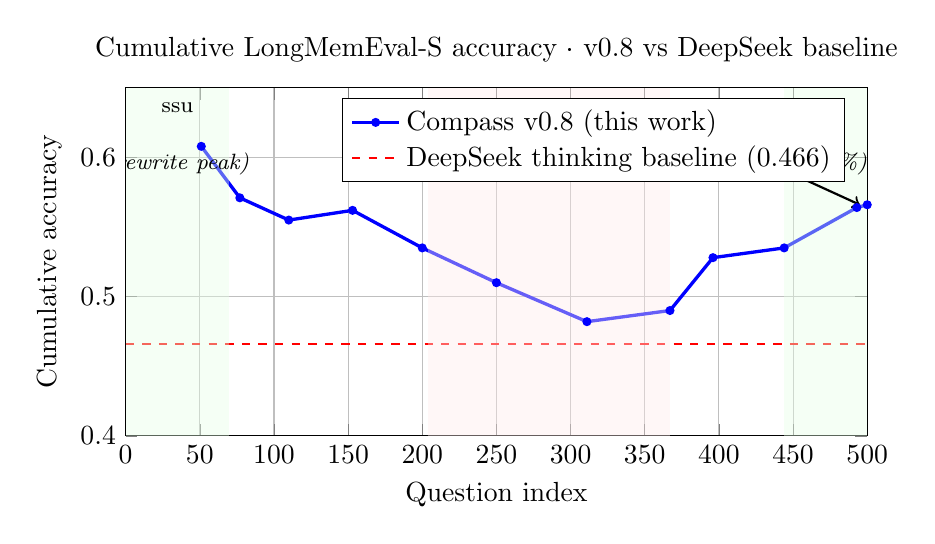
\begin{tikzpicture}
\begin{axis}[
    width=11cm, height=6cm,
    xlabel={Question index},
    ylabel={Cumulative accuracy},
    xmin=0, xmax=500,
    ymin=0.40, ymax=0.65,
    grid=major,
    legend pos=north east,
    legend cell align=left,
    title={Cumulative LongMemEval-S accuracy · v0.8 vs DeepSeek baseline}
]

% v0.8 trajectory (annotated peaks/troughs from RESULTS_v0.8.md)
\addplot[blue, very thick, mark=*, mark size=1pt] coordinates {
  (51, 0.608)
  (77, 0.571)
  (110, 0.555)
  (153, 0.562)
  (200, 0.535)
  (250, 0.510)
  (311, 0.482)
  (367, 0.490)
  (396, 0.528)
  (444, 0.535)
  (493, 0.564)
  (500, 0.566)
};
\addlegendentry{Compass v0.8 (this work)}

% Baseline (DeepSeek thinking · approx flat at 0.466)
\addplot[red, dashed, thick] coordinates {(0, 0.466) (500, 0.466)};
\addlegendentry{DeepSeek thinking baseline (0.466)};

% Question type bands (visual aids)
\fill[red!8, opacity=0.4] (axis cs:204,0.4) rectangle (axis cs:367,0.65);
\node[anchor=south, font=\footnotesize] at (axis cs:285, 0.605) {temporal-reasoning};
\node[anchor=south, font=\footnotesize\itshape] at (axis cs:285, 0.575) {(low V trough)};

\fill[green!10, opacity=0.4] (axis cs:0,0.4) rectangle (axis cs:70,0.65);
\node[anchor=south, font=\footnotesize] at (axis cs:35, 0.625) {ssu};
\node[anchor=south, font=\footnotesize\itshape] at (axis cs:35, 0.58) {(rewrite peak)};

\fill[green!10, opacity=0.4] (axis cs:444,0.4) rectangle (axis cs:500,0.65);
\node[anchor=south, font=\footnotesize] at (axis cs:472, 0.625) {ssa};
\node[anchor=south, font=\footnotesize\itshape] at (axis cs:472, 0.58) {(83.9\%)};

% Final value annotation
\node[anchor=south west, font=\footnotesize] at (axis cs:380, 0.610) {Final: \textbf{56.6\%}};
\draw[->, thick] (axis cs:415, 0.605) -- (axis cs:495, 0.566);

\end{axis}
\end{tikzpicture}
\end{document}
